\documentclass[11pt,a4paper]{article}

\usepackage{amsmath}
\usepackage{physics}
\usepackage[utf8]{inputenc}
\usepackage{graphicx}
\usepackage{biblatex}
\usepackage{float}

\addbibresource{References.bib}
\nocite{*}

\begin{document}

TITLE\\
AUTHORS\\
DATE

\cleardoublepage{}
\begin{abstract}
  
\end{abstract}
\cleardoublepage{}
\tableofcontents{}
\section{Introduction}
The standard model of particle is very successful at describing the fundamental
building blocks of our universe. It has been corroborated by numerous
experiments, but to further test the theory physicists collide particles
together at high energy to probe the produced debris from the collision, hoping
to discover new physics. A particle of particular interest is the top quark,
which is the heaviest known fundamental particle with a mass of
$173.34 \pm 0.27 \pm 0.71 \mathrm{GeV/c^2}$, and its coupling strength to all
the bosons are well predicted by the standard model. Because of this,
measurements of the top quark's properties plays an important role in testing
the Standard Model. Top quark production at LHC occurs via strong interactions,
where they are produced in top, anti-top pairs. One test of the Standard Model,
is the study of the $Wtb$ vertex Lorentz structure and coupling, which is
studied by looking at the decay products of top quarks. The top quarks decay,
with almost 100\% branching fraction, by weak interactions into $W$ bosons and
bottom quarks $t \rightarrow W + b$. The W bosons decay, into either a charged lepton and
neutrino; $W \rightarrow l + \nu_l$, or into a quark, anti-quark pair: $W \rightarrow q' + \bar{q}$.\\

\begin{figure}[H]
	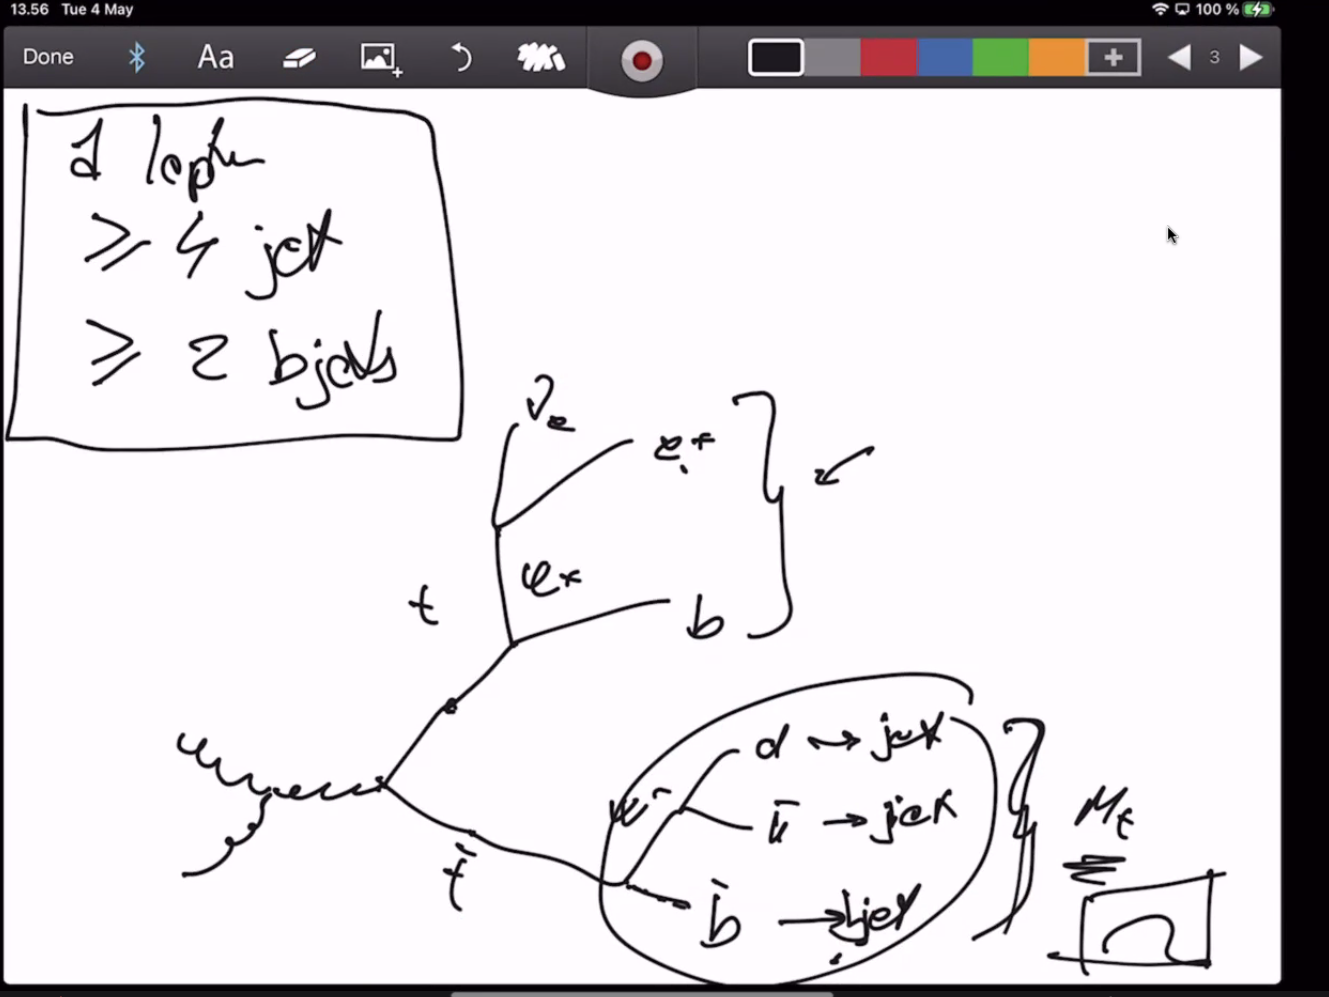
\includegraphics[width=\linewidth]{Placeholder_FeynmanDiagram.png}
	\caption{The Feynman diagram shows one of the possible decays of the top
      quarks. For this single leptonic decay, we see from the figure that there
      are 4 quark jets as the end product.}
	\label{fig_feynmandiagram}
\end{figure}

In this report, we are only looking at decays with a single lepton as decay
product. The leptons we look at are either electrons or muons, and the collision
will produce four jets, as evident from the diagram.


\subsection{Motivation}

\subsection{Top Quarks}

\section{Theory}

\subsection{Standard Model}
The Standard Model is a physical theory that unifies
three of the four fundamental forces, the electromagnetic force, the strong
force and the weak force. Attempts have been made to unify the standard model
with the final fundamental force, the gravitational force as described by
general relativity. These theories include loop quantum gravity and string
theory, however no experimental evidence has been gathered for either theory and
testing these theories is very difficult with our current measuring
equipment(?).\\
%"with current particle accelerators" måske?

The Standard Model contains all known elementary particles, they can be split
into fermions and bosons. Fermions can further be split up into Leptons and
Quarks. Fermions have spin $\frac{1}{2}$ and are grouped into three different
generations or families based on their masses, they obey the pauli-exclusion
principle which means that two identical fermions can't have the same quantum
numbers in a system. Each fermion has an antifermion with same mass but opposite
charge, colour and third component of weak isospin. \\
%that are split into two distinct categories, called fermions and bosons "is
%further split", eller bare "is split"

Bosons include the photon, gluon, W- and Z-boson. Which respectively are the
force carriers of the electromagnetic force, the strong force and the weak
force. Bosons unlike fermions don't obey the Pauli exclusion principle.
% måske lidt mere om kvarker (colour confinement) og kort beskrivelse til force
% carriers(?) (altså deres styrke, men ved ikke om det er vigtigt.
%jeg synes at det er en god intro og leder godt ind i afsnittet under om
%symmetries and laws of conservation.

\subsubsection{Quantum Chromo Dynamics}
Quantum chromo dynamics (QCD), is the theory of the strong interaction, which
binds the quarks together. In QCD, each quark is associated with a color charge,
that color confines the quark via the strong interaction, to other quarks, to
make up a total color charge of white. While the color charge isn't physically
related to actual colors, the way they mix together, is analogous to the way we
mix the colors green, red and blue, as well as their anti colors, magenta,
yellow and cyan. Because of these properties, quarks can bind together in groups
with odd number of quarks, with at least three, to form baryons, or an even
number of at least two, to form mesons.\\

If enough energy is added to stretch one of the quarks away from the rest, the
gluon field breaks, and a new quark and anti quark pair is created. This process
of creating new quark, anti quark pairs, by stretching the gluon field between
them is the result of violent inelastic collisions, which creates these jets of
quarks, anti quarks.

\subsubsection{Symmetries and Laws of Conservation} Emmy Noether showed that any
conservation law is associated with a continues symmetry of the Lagrangian. The
conservation laws of classical physics are the result of them being invariant
with respect to their canonically conjugate quantities. The conservation of
energy, linear momentum and angular momentum, stems from their invariance in
time, space and angles respectively. This implies that the laws of physics are
independent of the time, the location and the orientation in space.\\

Another symmetry, that is very important for quantum mechanics, is reflection
symmetry, called parity. A wave function can have positive or negative parity
depending on whether or not it changes sign under parity transformation. For the
laws which are invariant under reflection in space, the parity quantum number
$P$ is conserved, while in relativistic quantum mechanic, we need to ascribe an
intrinsic parity to particles and antiparticles.\\

Group theory gives us the tools to study these symmetries more elegantly, and
has become particularly useful to describe symmetries of quantum mechanics,
where degenerate eigenstates furnishes irreducible representations of a group.
In studying these groups, we can discover other conserved quantities in the
interactions of the electromagnetic (EM), the weak or the strong force.\\

The unitary group U(1), leads to conservation of charge in EM and strong
interactions, as well as the conservation of lepton number, as far as
we know in all interactions. Certain particles behave practically identically
with respect to the strong or the weak interactions, these properties are
studied through irreducible representations of the group SU(3), and are
characterized by strong and weak isospin, which are also conserved.\\

The Dirac equation extends the Schrödinger wave equations, to include the
effects of special relativity. The solution to this equation shows that for
relativistic particles, where $\beta = v/c \rightarrow 1$, the projection of a particle's spin
onto the direction of their momentum is conserved. This conserved quantity is
called helicity and is defined as

\begin{equation} h = \frac{\vb s \cdot \vb p}{\abs{\vb s} \cdot \abs{\vb p}}.
\end{equation}

Chirality is a fundamental property of a particle determined by representation
theory. In the relativistic limit the distinction between helicity and chirality
disappears, as the mass term $mc^2$ becomes negligible compared to the total
energy. The weak force will only interact with left-chiral particles and
right-chiral antiparticles. The operator of an interaction that describes the
exchange of a boson, can have both vector $V$ and axial vector $A$ nature. If it
has both a vector and an axial part as in the case of weak interactions parity
is violated while maximum parity violation occurs when both the contributions
becomes equal magnitude.

\subsection{Four-momentum}
The data collected in LHC collisions, allows us to reconstruct the 4-vector of
momentum for the involved particles. The 4-vector is a four component tensor,
made up of an ordinary 3-vector for relativistic momentum $\vb p$, and the
relativistic energy term, $E^2/c^2$, as its first component. Working in natural
units, where we set $c=1$, our 4-vector will be given as
\begin{equation}
p = \left(\begin{matrix} E^2 \\ \vb p \end{matrix} \right).
\end{equation}

The dot product of two 4-vectors is given by $p\cdot p' = E E' - \vb p \cdot \vb{p'}$,
where $\vb p \cdot \vb{p'}$ is the ordinary dot product of two 3-vector momentum.
From special relativity, we know that $E^2 - \abs{\vb p}^2 = m^2$, so from the
dot product, we get that $p^2 = m^2$. Other vector operations on a 4-vector is
similar to those same vector operations on a 3-vector. The quantity
\begin{equation}
s = (p + p')^2 = (E + E')^2 - (\vb p + \vb p')^2
\end{equation}

is conserved, and is the centre-of-mass energy squared of the system. It is the
energy available to create new particles, or probing the properties of
particles.

\subsection{Coupling of W$^+$bt}
The $W$boson couples only to left-handed particles, which gives $Wtb$ vortex a
(V-A) structure. In the Standard Model we expect that the $W$boson and $b$quark,
from top decay, arrange such that chiral structure of the couple vertex is
fulfilled. Because of parity violation, the events with positive helicity (right
polarized) gets suppressed, while events with negative (left polarized) and
longitudinal helicity dominates. The fraction of; longitudinally $F_0$, left
$F_L$ or right $F_R$ polarized $W-$bosons which are produced from top quark
decay, we refer to as helicity fractions. In the Standard Model we can determine
these fractions with quantum chromo dynamics, in next to next to leading order
calculations to be $F_0 = 0.687 \pm 0.005$, $F_L = 0.311 \pm 0.005$ and
$F_R = 0.0017 \pm 0.0001$. The experimental method to extract these fractions is
by studying the angular decay distribution of the leptonic decay products of the
top quark. The angular distribution is given by:

\begin{equation}
  \frac{1}{\Gamma}\dv{\Gamma}{\cos \theta^*} = \frac{3}{8}(1-\cos \theta^*)^2 F_L +
  \frac{3}{4}\sin^2 \theta^* F_0 + \frac{3}{8}(1+\cos \theta^*)^2 F_R.
\end{equation}

Where $\theta^*$ is the helicity angle, which is defined as the angle between the
decayed lepton momentum direction, and the reversible momentum direction of the
$b$-quark decay from the same top quark, viewed from a reference frame with $W$
at rest. From the 4-vectors of the lepton and $b$-jet, we can find the
$\cos \theta^*$ from the following expression:
\begin{equation}
  \cos \theta^* = \frac{p_e \cdot p_b - E_e E_b}{\abs{\vb{p_e}} \abs{\vb{p_b}}} \simeq
  \frac{2 M_{eb}^2}{m_t^2 - M_W^2} - 1,
\end{equation}

here $p_l$ and $p_b$ are the four momentum vectors of the lepton and the bottom
quark respectively. $M_{lb}$ is the invariant mass of the lepton and bottom
quark system.

\section{Apparatus}

\subsection{LHC}
In the Large Hadron Collider (LHC), top quarks are mainly produced through
violent collisions of protons, causing gluon-gluon fusion, which produces top,
anti-top pairs $gg \rightarrow t\bar t$. The data used in this paper, is from the 2016 run
at LHC, with a centre-of-mass energy of $\sqrt s = 13 \mathrm{TeV}$, which
corresponds to an integrated luminosity of 10 $\mathrm{fb}^{-1}$. At these
energies, the protons are accelerated close to the speed of light before their
collisions in the ATLAS detector.\\

This process starts, when protons are produced from hydrogen gas in a linear
accelerator LINAC2 then gets injected into the LHC, through a series of smaller
synchrotron accelerators, Proton Syncrotron Booster (PSB), Proton Syncrotron
(PS) and Super Protron Synhrotron (SPS). The LHC receives bunches from another
SPS, containing a lot of protons in each bunch, effectively increasing the
cross-sectional area for collisions to occur. In order to prevent energy loss
due to synchrotron radiation, the LHC was built to be the largest particle
accelerator in the world, which has allowed it to reach higher energies than
other accelerators. At these energies, more events happen inside the detector,
described by the following equation:
\begin{equation}
  N = \sigma \int L \dd t,
\end{equation}

where $N$ is the number of expected events, $\sigma$ is the cross-sectional area of
the events, and $\int L \dd t$ is the integrated luminosity.

\subsection{ATLAS}
% https://atlas.web.cern.ch/Atlas/TP/NEW/HTML/tp9new/tp9.html
% https://atlas.cern/discover/detector
% https://en.wikipedia.org/wiki/ATLAS_experiment#ATLAS_detector
% Gamle hjemmeside: https://web.archive.org/web/20110614103207/http://atlas.ch/detector.html

% potential figure https://commons.wikimedia.org/wiki/File:ATLAS_Drawing.jpg

The ATLAS detector consists of multiple primary components, each with their own
subcomponents or subsections.

\subsubsection{The Inner Detector}
% https://atlas.web.cern.ch/Atlas/TP/NEW/HTML/tp9new/node10.html#SECTION00433000000000000000
% https://atlas.cern/discover/detector/inner-detector
% https://en.wikipedia.org/wiki/ATLAS_experiment#Inner_Detector
The purpose of this component is to measure charge and momentum, including it's
direction, of the detected particle. It consists of three subcomponents.
\paragraph{Pixel Detector}
\paragraph{Semiconductor Tracker}
\paragraph{Transition Radiation Tracker.}

\subsubsection{Calorimeter}
% https://atlas.web.cern.ch/Atlas/TP/NEW/HTML/tp9new/node9.html#SECTION00432000000000000000
% https://atlas.cern/discover/detector/calorimeter
% https://en.wikipedia.org/wiki/ATLAS_experiment#Calorimeters
This component will stop particles moving through while measuring the
energy they lose by being stopped. % måske lidt kringlet og er passivt
The Calorimeter can not stop muons and neutrinos.

% 2 subcomponents
\paragraph{Liquid Argon Calorimeter}
\paragraph{Tile Hadronic Calorimeter}

\subsubsection{Muon Spectrometer}
% https://atlas.web.cern.ch/Atlas/TP/NEW/HTML/tp9new/node11.html#SECTION00434000000000000000
% https://atlas.cern/discover/detector/muon-spectrometer
% https://en.wikipedia.org/wiki/ATLAS_experiment#Muon_Spectrometer
This detects the muons, which have passed through the calorimeter and inner
detector, and measures their momenta.

\paragraph{Thin Gap Chambers}
\paragraph{Resistive Plate Chambers}
\paragraph{Monitored Drift Tubes}
\paragraph{Cathode Strip Chambers}

\subsubsection{Magnet System}
% https://atlas.web.cern.ch/Atlas/TP/NEW/HTML/tp9new/node8.html#SECTION00431000000000000000
% https://atlas.cern/discover/detector/magnet-system
% https://en.wikipedia.org/wiki/ATLAS_experiment#Magnet_system
This system bends the path of the particles, such that their track stays within
the confines of the detector.

\paragraph{Central Solenoid Magnet}
\paragraph{Barrel Toroid}
\paragraph{End-cap Toroids}

\subsubsection{Data Collection}
% https://atlas.web.cern.ch/Atlas/TP/NEW/HTML/tp9new/node12.html
% https://en.wikipedia.org/wiki/ATLAS_experiment#Data_systems
% https://atlas.cern/discover/detector/trigger-daq
The detector generates 60 terabytes of data per second from the 1.7 billion
collisions taking place in the detector in that time frame. Therefore, The ATLAS
Detector has a hardware trigger system which helps selectively save only data in
which a particle has been detected.

% HLT = CPU farm but not trigger? data compiler?

\section{Monte Carlo Simulation}
Monte Carlo (MC) simulation was used to model the signal and background
processes expected at the LHC, for the 13 TeV Atlas Open Data used for this
report. This process follows four steps, starting with an event generation which
uses a MC generator to mimic the initial pp collision. In the second step,
detector simulation, the geometry of the ATLAS detector and its material
properties gets simulated. As part of the digitisation step, the previous step
is followed by simulating the responding signals in read-out data written in a
format compatible with real output of the detector. Finally these data can be
used to reconstruct the collisions, particle trajectories and subsequent products.\\

In The 13 TeV ATLAS Open Data set, there are several SM processes which are
modelled using MC simulations. For the purpose of this report, the MC
simulations on top-quark-pair production was used alongside real data taken from
the detector, to compare theory with real data.

\section{Data Analysis}
% Definer Psuedorapidity \eta %
% http://opendata.atlas.cern/release/2020/documentation/physics/SL3.html
\subsection{Event Selection}
In order to identify the top-quark-pair production, several cuts in the data were implemented. The criteria are as follows 
\begin{itemize}
	\item Only one electron or muon in the final state with $p_{T} > 30 \mathrm{GeV}$
	\item Missing transverse momentum $E_{T}^{miss} > 30 \mathrm{GeV}$
	\item Transverse mass of the W-boson $M_{T}^{W} > 30 \mathrm{GeV}$
	\item At least four jets with $p_{T} > 30 \mathrm{GeV}$, with two of these being b-tagged
	\item Electrons are required to have $|\eta| > 2.47$ aside from $1.37 < |\eta| < 1.52$
	\item Muons are limited by $|\eta| > 2.50$
\end{itemize}
where $\eta$ describes angle between the particle and the beam axis given by 
\begin{equation}
	\eta = -\ln({\tan\left(\frac{\theta}{2}\right)})
\end{equation}
\subsubsection{B-tagging}
%\subsubsection{Single Lepton Channel}

\subsection{The Code}

\subsubsection{ROOT}

\subsection{Results}

\section{Conclusion}

\printbibliography

\end{document}
